
\section{Introduction}
This is the report to the databases project, taken in the fall semester 2018. At first, the problem setting, the chosen data sources and the posed questions are introduced. Following, the single source schemas and the integrated schema provide an overview of the existent data and their derived relations. After an insight into the used methods for the integration and analysis, this report is concluded with the results and lessons learned.

\subsection{Problem Setting}
The project tasks are split into four parts:
\begin{itemize}
	\item \textbf{Project idea:} Select multiple data sources and pose analysis goals
	\begin{itemize}
		\item Select two to three interesting data sources
		\item In various sizes, formats and from multiple sources
	\end{itemize}
	\item \textbf{Schema integration:} Analyse the data sources and design an integrated schema
	\begin{itemize}
		\item Analyse data sources
		\item Create entity relationship diagrams of single sources
		\item Create entity relationship diagram of integrated schema with derived relations
	\end{itemize}
	\item \textbf{Data integration:} Integrate the data sources into a unified and normalized database
	\begin{itemize}
		\item Integrate the data into the global schema
		\item Perform cleaning and normalization
		\item Create necessary index structures
	\end{itemize}
	\item \textbf{Analysis and visualization:} Use the reconciled data for performing analyses and creating visualizations
	\begin{itemize}
		\item Use analysis queries and visualizations to achieve the analysis goals
	\end{itemize}
\end{itemize}



\subsection{Goals}
The goal of this project is to answer the following questions:
\begin{itemize}
	\item Are terror events dependent on the weather?
	\item Do terror attacks influence founding/splitting of metal bands and vice versa?
	\item Does the population influence the number of existing metal bands?
	\item Do terror attacks have an influence on the population?
	\item Which main genre has the most terror events?
\end{itemize}

\section{Sources}
Four data sources were chosen for this project. The global terrorism data source was selected at first, followed by population and metal bands. The idea of weather having an influence on terrorism occurred and a fitting weather source was select in addition to the others.

This section provides a short introduction to the single data sources.

\subsection{Global Terrorism 1970 - 2017}
\begin{itemize}
	\item URL: \url{https://www.kaggle.com/START-UMD/gtd}
	\item Dimensions: 181'691 rows x 135 columns
	\item Size: 162.8 MB
	\item Format: CSV
\end{itemize}

This data set contains a list of global terror events, beginning in 1970 and ending in 2017. The events state a location, time and descriptions of attack groups, targets, weapons used, etc.. 
	
\subsection{Metal bands 1964 - 2016}
\begin{itemize}
	\item URL: \url{https://www.kaggle.com/mrpantherson/metal-by-nation# metal_bands_2017.csv}
	\item Dimensions: 5000 rows x 7 columns
	\item Size: 264 KB
	\item Format: CSV
\end{itemize}

Here, 5000 metal bands are listed with the country they originate from, when they were formed and when they split up. Additionally, one or multiple metal styles are given for each band.

\subsection{World Population 1960 - 2015}
\begin{itemize}
	\item URL: \url{https://www.kaggle.com/mrpantherson/metal-by-nation#world_population_1960_2015.csv}
	\item Dimensions: 264 rows x 57 columns
	\item Size: 125 KB
	\item Format: CSV
\end{itemize}

This data set contains the population of 264 countries for each year, starting in 1960 and ending in 2015.

\subsection{Weather Data}
\begin{itemize}
	\item URL: \url{ftp://ftp.ncdc.noaa.gov/pub/data/ghcn/daily/}
	\item Inventory
	\begin{itemize}
	  \item Dimensions: 65236 rows x 6 columns
	  \item Size: 26.9 MB
	  \item Format: TXT
    \end{itemize}
	\item Daily
	\begin{itemize}
	  \item Dimensions: $\sim$10M rows x 35 columns
	  \item Size: 2.9 GB
	  \item Format: DLY
    \end{itemize}
\end{itemize}

The inventory file contains information about the time span of measurements, location and id of all weather station from the National Oceanic and Atmospheric Administration. After the relevant stations are found, their measured data can be found in the \texttt{dly} file, which has the same name as the station id. The data consists of daily means of multiple elements (such as temperatures, precipitation, snow fall, etc.) for the whole time span the station was active.

\subsection{Single source ER diagram}
Figure \ref{fig:singlesource} shows the ER diagram of the introduced data sets. 

\begin{figure}[hbt!]
	%\centering
    \subfloat[Metal\label{fig:metal}]{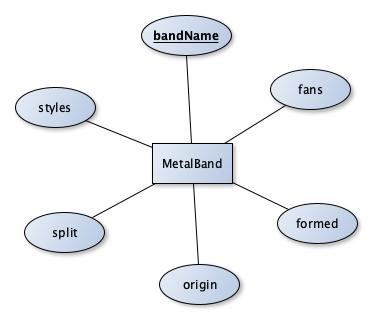
\includegraphics[width=0.45\textwidth]{g2-metal.jpg}}\qquad
    \subfloat[Country\label{fig:country}]{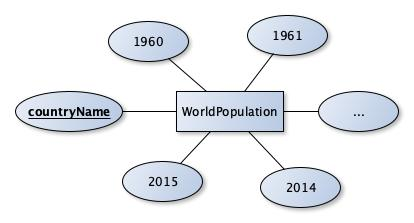
\includegraphics[width=0.45\textwidth]{g2-country.jpg}}\qquad
    \centering
    \subfloat[Terrorism\label{fig:terrorism}]{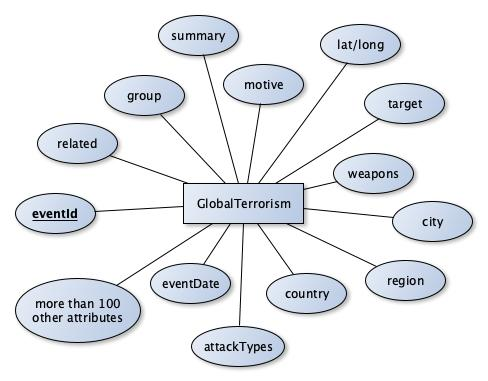
\includegraphics[width=0.65\textwidth]{g2-terror.jpg}}\qquad\\
    \centering
    \subfloat[Weather\label{fig:weather}]{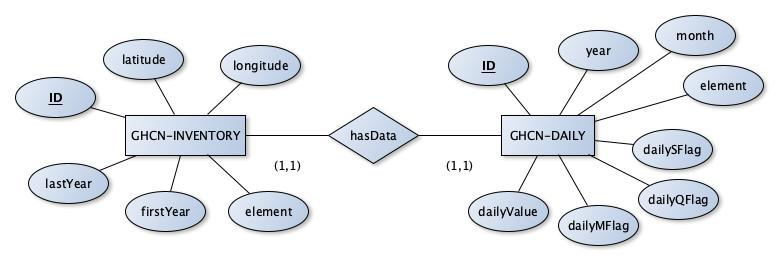
\includegraphics[width=\textwidth]{g2-weather.jpg}}\qquad
    \caption{Entity-Relation diagrams of single sources}
\label{fig:singlesource}
\end{figure}

\section{Integrated Schema}
A new population entity replaces the year attribute in \texttt{Country}. Some of the terror data is outsourced to new entities, as some attributes are listed data points. A new entity \texttt{TerrorLocation} is created to simplify relations with countries and weather data.

\subsection{ER}
\begin{figure}[hbt!]
	\centering
	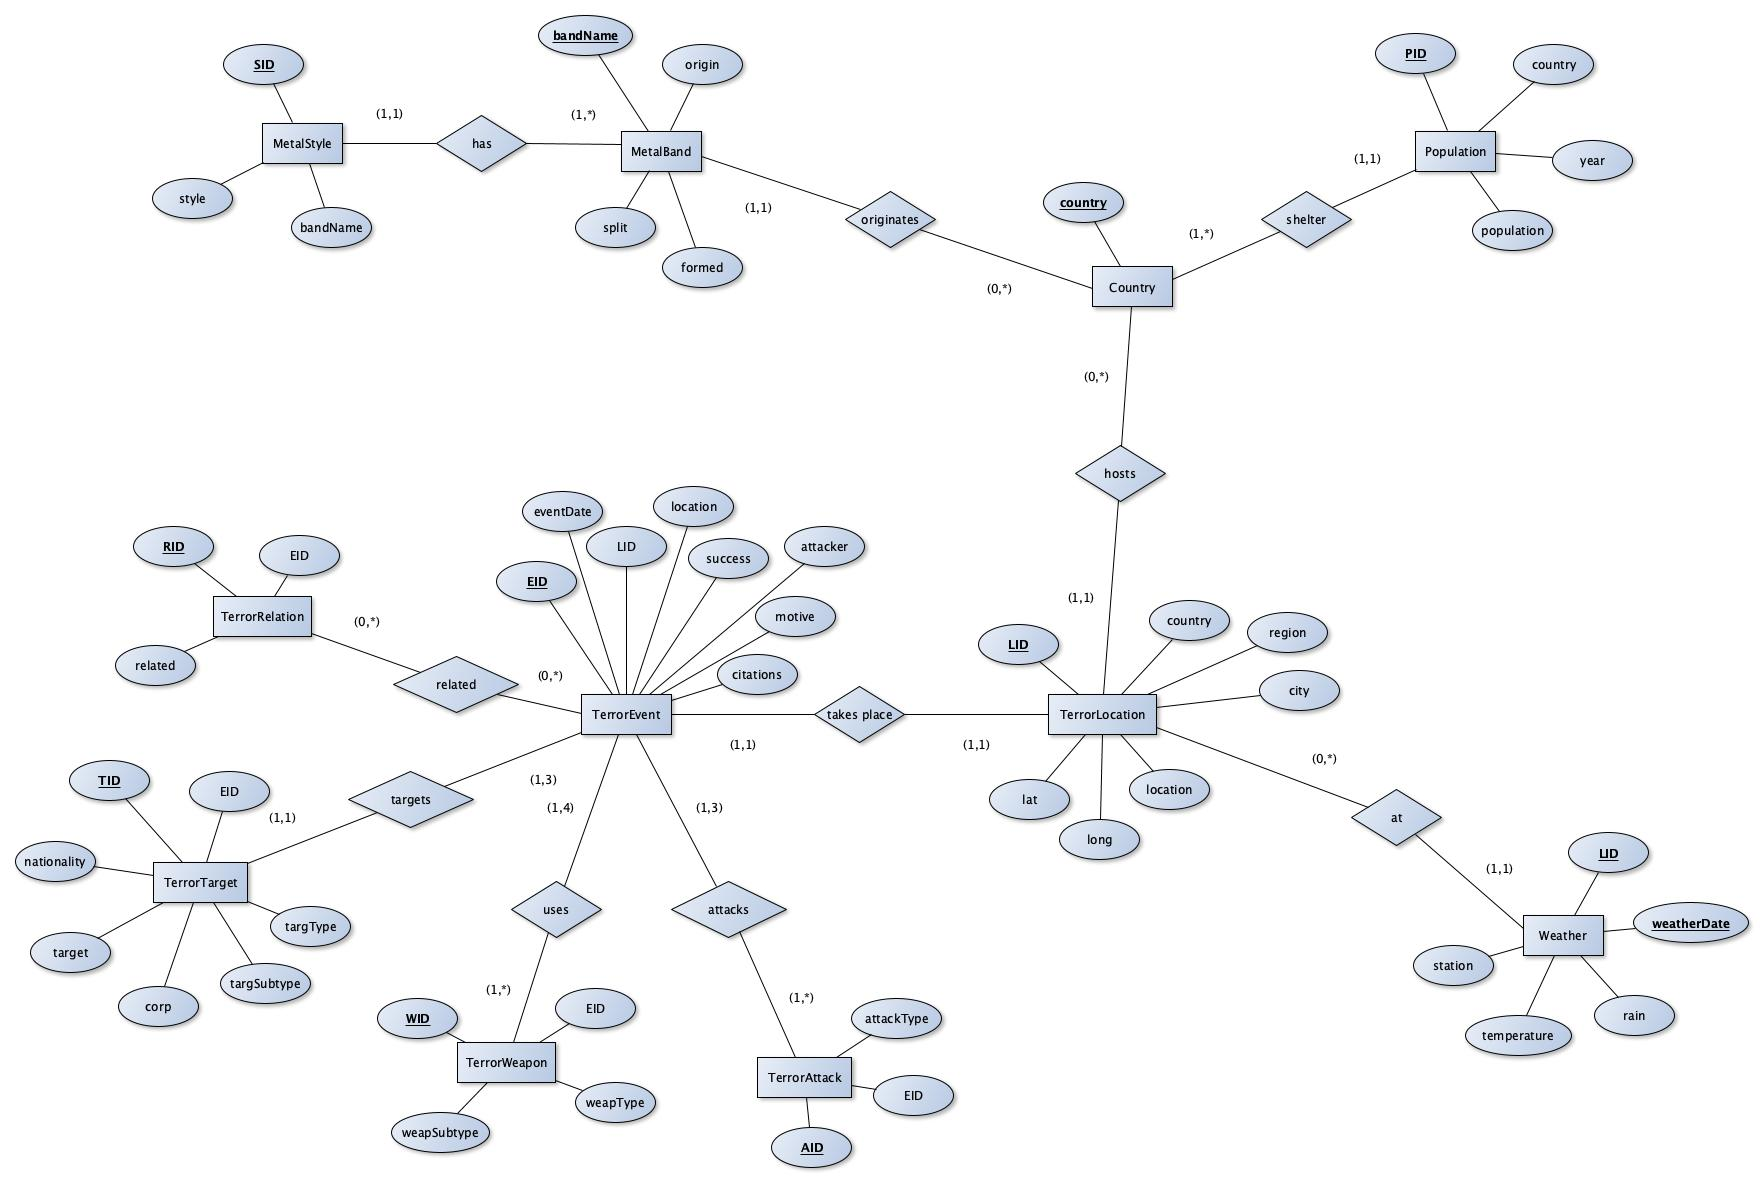
\includegraphics[width=1.4\textwidth, angle=270]{g2-integratedSchema.jpg}
	\caption{Entity-Relation diagram integrated schema}
\end{figure}
    
\subsection{Logical Schema}
\begin{itemize}
\item Country (\underline{countryName})
\item MetalBand (\underline{bandName}, formed, \uwave{origin}, split)
\item MetalStyle (\underline{SID}, \uwave{bandName}, style)
\item Population (\underline{PID}, \uwave{country}, year, population)
\item TerrorAttack (\underline{AID}, \uwave{EID}, attackTypeID, attackType)
\item TerrorEvent (\underline{EID}, eventDate, approxDate, extended, resolution, \uwave{LID}, summary, crit1, crit2, crit3, doubtterr, alternativeID, alternative, multiple, success, suicide, nkill, nkillus, nkillter, nwound, nwoundus, nwoundte, property, propextentID, propextent, propvalue, propcomment, addnotes, weapdetail, gname, gsubname, gname2, gsubname2, gname3, gsubname3, motive, guncertain1, guncertain2, guncertain3, individual, nperps, nperpcap, claimed, claimmodeID, claimmode, claim2, claimmode2ID, claimmode2, claim3, claimmode3ID, claimmode3, compclaim, ishostkid, nhostkid, nhostkidus, nhours, ndays, divert, country, ransom, ransomamt, ransomamtus, ransompaid, ransompaidus, ransomnote, hostkidoutcomeID, hostkidoutcome, nreleased, scite1, scite2, scite3, dbsource, INT\_LOG, INT\_IDEO, INT\_MISC, INT\_ANY)
\item TerrorLocation (\underline{LID}, countryID, \uwave{country}, regionID, region, provstate, city, latitude, longitude, specificity, vicinity, location)
\item TerrorRelation (\underline{RID}, \uwave{EID}, {related})
\item TerrorTarget (\underline{TID}, \uwave{EID}, targTypeID, targType, targSubtypeID, targSubtype, corp, target, nationalityID, nationality)
\item TerrorWeapon (\underline{WID}, \uwave{EID}, weapTypeID, weapType, weapSubtypeID, weapSubtype)
\item Weather (\underline{\uwave{LID}, weatherDate}, rain, temperature, station)
\end{itemize}

